\newpage

\section{فصل هشتم}

در این فصل و فصل‌های بعدی در مورد نمایش بصری اهداف، ریسک‌ها و تمام مطالبی که در
فصل‌های پیشین خوانده‌ایم می‌پردازیم. این فصل تکنیک‌هایی را برای مدل سازی
سیستم‌هایی با اهداف \lr{FR} و \lr{NFR} را مطرح می‌کند. در کتاب مرجع ریسک‌ها را
به نام \lr{Obstacles} می‌شناسند.

نیازمندی سیستم یا \lr{System requirement} یک هدف چند عامله و \lr{Software
requirement} یک هدف تک عامله می‌باشد. یکسری اهداف استراتژیک وجود دارد که به
اهداف کوچک‌تری ریز می‌شوند تا قابل فهم مهندس نیازمندی باشند. از اشکال هندسی برای
بیان اهداف و زیر مجموعه آنها، برگ‌ها و غیره استفاده می‌کنیم.

\subsection{اهداف}

شکل متوازی الاضلاع اهداف را مشخص می‌کند.

\begin{figure}[H]
    \centering
    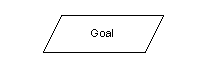
\includegraphics[width=0.5\textwidth]{assets/goal.drawio.pdf}
    \caption{یک هدف}
\end{figure}

\subsection{پر رنگ بودن متوازی الاضلاع}

پر رنگ شدن یا \lr{Bold} شدن اشکال برای نشان دادن برگ‌ها، \lr{Assumption}ها و
نیازمندی‌های سیستم است به آن معنا که دیگر شکست و مشتق گرفتن در آن قسمت نخواهیم
داشت و آن مورد آخرین نود در نمودار خواهد بود.

\begin{figure}[H]
    \centering
    
\includegraphics[width=0.5\textwidth]{assets/complete_goal.drawio.pdf}
    \caption{برگ‌هایی که بعد از آن دیگر شکست اتفاق نمی‌افتد.}
\end{figure}

\subsection{کامل بودن یا کامل نبودن \lr{Complete}}

\begin{itemize}
    \item نقاط تو پر کامل بودن را مشخص می‌کنند. دقیقاً جایی که شکست متوقف
    می‌شود.
    \item نقاط تو خالی ادامه‌دار بودن مشتقات زیرین را مشخص می‌کنند.
\end{itemize}

\begin{figure}[H]
    \centering
    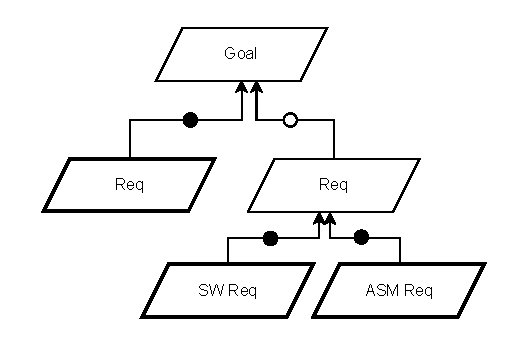
\includegraphics[width=0.6\textwidth]{assets/complete.drawio.pdf}
    \caption{قابل مشتق بودن یا نبودن یک نیازمندی با پر رنگ شدن و \lr{Bold} شدن.}
\end{figure}

\subsection{مواردی توصیفی}

تمام موارد توصیفی‌ها (\lr{Descriptive}ها) مانند \lr{Domain proper} ها با با
ذوزنقه نمایش داده می‌شود.

\begin{itemize}
    \item سرعت قطار مخالف با صفر باشد و در‌های آن قفل باشد. به عنوان دامنه هدف
    محسوب می‌شود.
    \item اشکال توصیفی، هدف (\lr{Goal}) نیستند.
\end{itemize}

\begin{figure}[H]
    \centering
    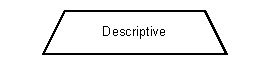
\includegraphics[width=0.5\textwidth]{assets/descriptive.drawio.pdf}
    \caption{عوامل توصیفی}
\end{figure}

\subsection{\lr{Domain properties}}

ویژگی‌های دامنه را با علامت خانه یا \lr{Home} نمایش می‌دهیم.

\subsection{عامل‌ها}

\lr{Goal} یک جمله می‌باشد و می‌تواند به دو صورت زیر باشد:

\begin{itemize}
    \item \lr{Multi-agent}: چند عامله
    \item \lr{Single-agent}: تک عامله
\end{itemize}

عامل یعنی آن المانی که \lr{Goal} را محقق می‌کند.

\begin{itemize}
    \item اگر هدف، \lr{System requirement} بود یعنی چند عامله می‌باشد.
    \item اگر هدف \lr{Assumption} و \lr{Software requirement} بود یعنی تک
    عامل هستند.
\end{itemize}

\begin{itemize}
    \item عامل شامل افراد، دستگاه‌ها و سنسور‌ها یا تمام کتابخانه‌ها و نرم‌افزاری
    موجود در حال حاضر
    \item برگ‌ها تک عامله هستند.
    \item عوامل را با ۶ ضلعی نمایش می‌دهیم.
\end{itemize}

\begin{figure}[H]
    \centering
    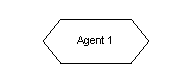
\includegraphics[width=0.5\textwidth]{assets/agent.drawio.pdf}
    \caption{نمایش یک عامل}
\end{figure}

\subsection{استاندارد نوشتاری هدف}

اهداف استاندارد نوشتاری دارند که به دو دسته زیر تقسیم می‌شوند:

\begin{enumerate}
    \item رفتاری
    \begin{itemize}
        \item \lr{Achieve}
        \item \lr{Maintain/Avoid}
    \end{itemize}
    \item نرم
\end{enumerate}

به طور کلی این استاندارد‌های نوشتاری را برای نوشتن گزاره‌ها استفاده می‌کنیم.

\subsubsection{اهداف رفتاری \lr{Achieve}}

اهداف \lr{Achieve} به اهدافی اطلاق می‌شود که یک سیستم باید به آن‌ها دست یابد یا
به تحقق آن‌ها کمک کند. این اهداف معمولاً توصیف‌کننده نتیجه‌ای هستند که سیستم
باید به دست آورد.

\subsubsection*{ویژگی اهداف \lr{Achieve}}

\begin{enumerate}
    \item توصیف‌کننده نتیجه نهایی هستند: این اهداف بیان می‌کند که سیستم می‌خواهد
    به چه چیزی برسد؟
    \item مثبت و سازنده هستند.
\end{enumerate}

\subsubsection*{مثال‌ها:}

\begin{itemize}
    \item سیستم باید قابلیت پردازش ۱۰۰۰ تراکنش را در ثانیه داشته باشد.
    \item سیستم باید اطلاعات کاربران را در کمتر از ۲ ثانیه بازیابی کند.
    \item قطار به سرعت ۱۲۰ کیلیومتر در ساعت رسید به مدت ۱۰ ثانیه بوق بزند. رسیدن
    به یک مقداری از سرعت باعث دیده شدن هدف رفتاری \lr{Achieve} شود.
    \item ظرفیت اشغال شده فایل‌ها در حافظه به ۱۲۰ گیگ رسید، یک اعلان در اعلانات
    کاربر ارسال کن و او را از پر شدن حافظه داخلی خود مطلع کن.
    \item قطار به خط قرمز رسید بوق بزند.
    \item در ماشین خودران، اگر چراغ قرمز را دیدی بایست.
    \item در فرمان‌های برقی، اگر سرعت بیشتر از ۲۰ کیلومتر در ساعت شود، فرمان از
    حالت نرم به حالت سفت و سخت تغییر دهد.
    \item سنسور باران، هنگام باران، برف پاک کن را فعال کند.
    \item در پیامرسان، هنگام تحویل پیام از فرستنده، علامت تیک را به پیام فرستند
    اعمال کن.
    \item پهنای باند در هنگام افزایش ترافیک سایت بیشتر شود.
\end{itemize}

\begin{algorithm}
    \caption{شبه‌کد بررسی سرعت قطار}
    \label{alg:trainSpeedAlgo}
    \begin{LTR}
        \begin{algorithmic}
            \State $trainSpeedStream \gets onlineTrainSpeedValue$
            \State $trainSpeed \gets 0$

            \While{$trainSpeedStream$}
                \If{$trainSpeed$ == $120Km/h$}
                    \State $beep \gets$ $for 10s$;
                \EndIf
            \EndWhile
        \end{algorithmic}
    \end{LTR}
\end{algorithm}

\subsubsection{اهداف رفتاری \lr{Maintain/Avoid}}

اهداف \lr{Maintain/Avoid} به اهدافی اطلاق می‌شود که سیستم باید وضعیت فعلی را حفظ
کند (\lr{Maintain}) یا از وقوع وضعیت خاصی جلوگیری کند (\lr{Avoid}).

\subsubsection*{ویژگی اهداف \lr{Maintain/Avoid}}

\begin{enumerate}
    \item حفظ وضعیت موجود یا جلوگیری از وقع پدیده‌ای
    \item منفی یا پیشگیرانی: اهداف \lr{Maintain} معمولاً به صورت حفظ وضعیت جاری
    فعالیت می‌کنند. اهداف \lr{Avoid} به صورت جلوگیری از وضعیت نامطلوب تعریف
    می‌شوند.
\end{enumerate}

\subsubsection*{مثال \lr{Maintain}:}

\begin{itemize}
    \item سیستم باید دسترسی مداوم به داده‌ها را حفظ کند.
    \item سرور اصلی شرکت بایستی ۲۴ ساعت و ۷ روز هفته در دسترس باشد.
    \item قطار حرکت کرد در‌ها قفل بمانند.
\end{itemize}

\subsubsection*{مثال \lr{Avoid}:}

\begin{itemize}
    \item اطلاعات قرض‌گیرندگان کتاب برای هیچ کس آشکار نشود.
    \item در برنامه فرانت، هنگام ورود گذرواژه، متن گذرواژه را مخفی کن.
    \item بعد از خاموش شدن خودرو، فرمان‌های برقی قفل شوند.
\end{itemize}

\subsubsection{اهداف نرم}

وقتی می‌گوییم بار کاری پرسنل \lr{Minimum} شود در حقیقت به هدف نرم اشاره داریم.
در این هدف عملی دیده می‌شود که یا مداوم انجام می‌شود یا برای یک لحظه انجام
می‌شود.

برای مثال، صفحه‌ای می‌خواهیم طراحی کنیم که برای کاربران نابینا قابل استفاده باشد
که آن را به شکل زیر می‌نویسیم:

$Max(usability)$

هر چقدر بیشتر باشد قابلیت استفاده از آن برای کاربران نابینا بیشتر می‌شود.

یا به عنوان مثال هزینه تولید نرم‌افزار کاهش یابد:

$Min(costs)$

یا به عنوان مثالی دیگر، مصرف \lr{CPU} کاهش یابد:

$Min(cpu usage)$

اهداف نرم اولویت‌بندی می‌شوند و از بین آن‌ها یک یا دو گزینه انتخاب می‌شود.

\subsubsection{نکته بین اهداف نرم و \lr{Avoid}}

آیا همه اهداف نرم به صورت \lr{NFR} هستند؟

خیر، برای مثال بخش \lr{Avoid} که در مورد عدم اطلاع از اطلاعات قرض‌گیرنده کتاب
است، یک روش امنیتی است ولی به صورت \lr{NFR} دیده نمی‌شود بلکه در واقع به صورت
رفتاری می‌باشد.

\subsection{استیت‌ها}

متغیر‌ها یا \lr{state}ها صفاتی خاص هستند با مقادیری خاص. نکته مهم آن است که
عوامل یا \lr{Agents} مسئول تغییر مقادیر این استیت‌ها هستند.

برای مثال سنسور در به عنوان یک \lr{Assumption} در نظر گرفته می‌شود که یک عامل به
نام سنسور دارد که این عامل وظیفه دارد مقدار \lr{doorStatus} را صفر یا یک کند که
صفر به معنای بسته بودن و یک به معنای باز بودن است. بعد از تغییر استیت آن را در
ساختمان داده مربوطه قرار می‌دهد.

\subsection{نمونه‌ای از دیاگرامی که شامل تضاد است}

% TODO: Draw conflict diagram here

\subsection{نکات تکمیلی}

\begin{itemize}
    \item برای انتخاب بین دو شاخه از \lr{SysRef} استفاده می‌شود که بین دو انتخاب
    اگر یک انتخاب داشته باشیم می‌تواند به \lr{System-to-be} تبدیل شود. در حقیقت
    همان تصمیم قبلی می‌باشد که در حال داریم استفاده می‌کنیم.
    \item در نمودار ممکن است \lr{System-as-is} داشته باشیم یعنی چیزی باشد که
    اکنون در حال استفاده از آن هستیم و جز \lr{Assumption}های ما می‌باشد.
\end{itemize}

\subsection{بخش \lr{Annotation}ها}

برای توضیح یک هدف از \lr{Annotation} استفاده می‌کنیم که در آن یکسری مشخصات هدف
نوشته می‌شود تا توضیحات و مستندات بیشتری در مورد آن هدف وجود داشته باشد. تمام
\lr{Annotation}ها در داخل مستطیل نقطه چین نوشته می‌شوند. نوشتن این ویژگی‌ها در
هر نموداری متفاوت است و شرایط لازم خودش را داراست. برای مثال در نمودار هدف فقط
دو ویژگی الزامی است ولی در نمودار ریسک بایستی ویژگی‌های بیشتری را به صورت الزامی
در این سند متذکر شویم. این مشخصات و ویژگی‌ها به ترتیب زیر هستند:

\subsubsection{ویژگی نام یا \lr{Name}}

این ویژگی ضروری است و در حقیقت نام هدف را به صورت کامل می‌نویسد. گاهی ممکن است
در متوازی‌الاضلاع بخواهیم به صورت سر کلمه یا خیلی خلاصه هدف را بنویسیم، در اینجا
می‌توانیم اسم کامل هدف را بنویسیم.

\subsubsection{ویژگی تعریف یا \lr{Definition}}

این ویژگی ضروری است چرا که باید تعریف کاملی از هدف را در آن بنویسیم تا به طور
واضح هدف مشخص شود تا در سری بعدی هیچ ابهامی برای درک آن نداشته باشیم.

\subsubsection{ویژگی نوع یا \lr{Type}}

این ویژگی اختیاری است. در این ویژگی مشخص می‌کنیم نوع هدف چیست. هدف رفتاری است یا
نرم؟

\subsubsection{ویژگی دسته‌بندی یا \lr{Category}}

این ویژگی اختیاری است. دسته‌بندی نوع هدف را مشخص می‌کند که از نوع عملیاتی
\lr{FR} است یا غیر-عملیاتی \lr{NFR}.

\subsubsection{ویژگی منبع یا \lr{Source}}

این ویژگی اختیاری است. منبع یا منابعی که از هدف مورد نظر مشخص شده است را
می‌نویسیم. مهم‌ترین کاربرد آن این است که اگر سوالی وجود داشته باشد یا ابهامی
مطرح شود که در نسخه‌های بعدی بایستی آن را تغییر دهیم سریع بتوانیم آن را پیدا
کنیم و در نسخه‌های بعدی آن را بهبود دهیم.

\subsubsection{ویژگی اولویت یا \lr{Priority}}

این ویژگی اختیاری است. در حقیقت برای تعیین اولویت از همان نمودار \lr{AHP}
استفاده می‌کنیم و آن را به صورت مستند روی دیاگرام نمایش خواهیم داد.

\subsubsection{ویژگی مسئله یا \lr{Issue}}

\begin{itemize}
    \item این ویژگی اختیاری است. زمانی که در حال مستندسازی هستیم ممکن است برای
    ما سوالی پیش آید که ابهام داشته باشد. برای مثال قطار‌هایی که در داخل سیستم
    تعریف شده‌اند را هر چند وقت یکبار باید تعمیرات و نگهداری کنیم؟ کدام از آنها؟
    آن‌هایی که در انبار هستند یا آن‌هایی که در حال استفاده می‌باشند؟ باید یک
    دسته از \lr{Issue} درست کنیم که مانند یک چک نویس مرتب و منظم بدانیم که هر
    موقع چه اتفاقی باید بیوفتد.
    \item در ضمن هر قسمتی که در منبع نوشته شده باشد می‌تواند به ما در حل کردن
    \lr{Issue} کمک کند.
    \item معمولاً مسائل و \lr{Issue} را زمانی بررسی می‌کنیم که تعدادشان زیاد شده
    باشد تا بتوانیم نسبت به همه ابهاماتمان را برطرف کنیم.
\end{itemize}

\subsubsection{ویژگی \lr{Formal specification}}

این ویژگی اختیاری است. ما می‌توانیم از زبان و گرامر رسمی یا \lr{Formal} استفاده
کنیم که یک زبان منطقی را استفاده می‌کند و باید سیستم عملیات بحرانی را آموخته
باشیم. برای مثال می‌توان در این قسمت از زبان \lr{Z} یا \lr{CSP} استفاده نمود.

\subsubsection{ویژگی معیار برازنده یا \lr{Fit criterion}}

این ویژگی اختیاری است. این ویژگی تنها برای اهداف نرم یا \lr{Soft goals} کار
می‌کند. در بخش‌های قبلی مثالی را آورده‌ایم که «بار کاری باید کمینه شود» چقدر
باید کمینه شود تا مهندس نیازمندی را راضی کند؟ نمی‌توانیم تنها بگوییم که کاهش
یابد، بایستی بیان کنیم که چقدر کاهش یابد؟ این ویژگی سنجشی برای آن دسته از اهداف
نرم می‌باشد. مقدار و مفهوم کیفی را کمی‌سازی می‌کند و مفهوم کیفی \lr{Soft goal}
می‌باشد.

\begin{figure}[H]
    \centering
    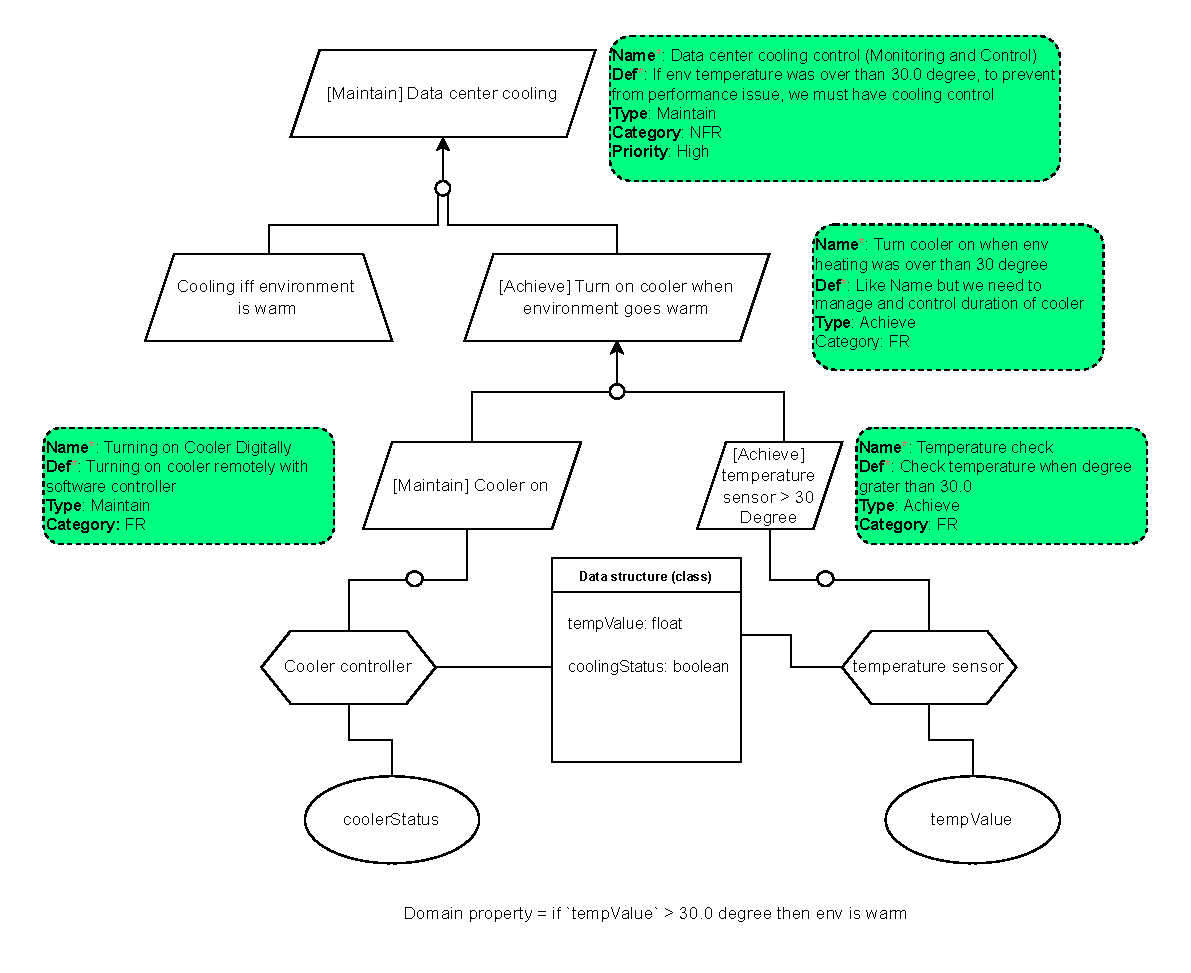
\includegraphics[width=0.5\textwidth]{assets/exp_1.drawio.pdf}
    \caption{نمونه‌ای از نمودار هدف که شامل عامل، ویژگی دامنه، تغییر وضعیت و
    ساختار داده می‌باشد.}
\end{figure}
